La strategia di progettazione del design che è stata implementata è \emph{Responsive Web Design}.\\
Questa tecnica è incentrata sull'accessibilità e permette la realizzazione del sito in modo che si possa adattare graficamente in modo automatico al tipo di device che si sta utilizzando.\\ 
Il layout che è stato scelto è un \emph{layout a cinque pannelli}, che si adatta facilmente al concetto di \emph{Responsive Web Design}.\\
I pannelli presenti nel layout sono, in ordine di presentazione:
\begin{enumerate}
	\item \textbf{header:} contiene il logo della pasticceria e un titolo che descrive la pagina corrente;
	\item \textbf{breadcrumb:} contiene il percorso della pagina corrente, serve ad orientare l'utente all'interno del sito;
	\item \textbf{menu:} contiene le varie sezioni del sito: quella corrente appare in grassetto, mentre le sezioni già visitate sono contrassegnate in viola. Inoltre, sotto le voci del menu corrispondenti alle sezioni, 
	appaiono due box con informazioni relative alle news e agli orari della pasticceria;
	\item \textbf{content:} contiene il contenuto della pagina corrente;
	\item \textbf{footer:} contiene le informazioni riguardo i contatti, gli orari della pasticceria, il form per accedere all'\emph{Area Amministratore}, i progettisti del sito, il copyright e gli standard rispettati.
\end{enumerate}

\newpage
Il layout si presenta in modi diversi, in base alle dimensioni dello schermo sulla quale l'utente sta navigando:\\
\begin{itemize}
	\item
	\textbf{Versione desktop}\\ 
	\begin{figure}[!h]
		\centering
		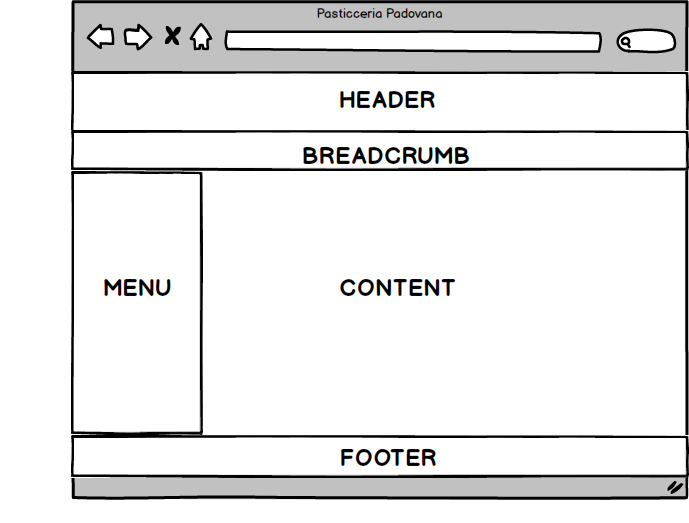
\includegraphics[width=0.7\linewidth]{sezioni/Progettazione/Immagini/desktop_layout.png}
	    \caption{Layout di una pagina in versione desktop}
		\label{Fig:verDesktop}
	\end{figure}
	\item	  
	\textbf{Versione mobile}	
	\begin{figure}[!h]				  
		\centering
		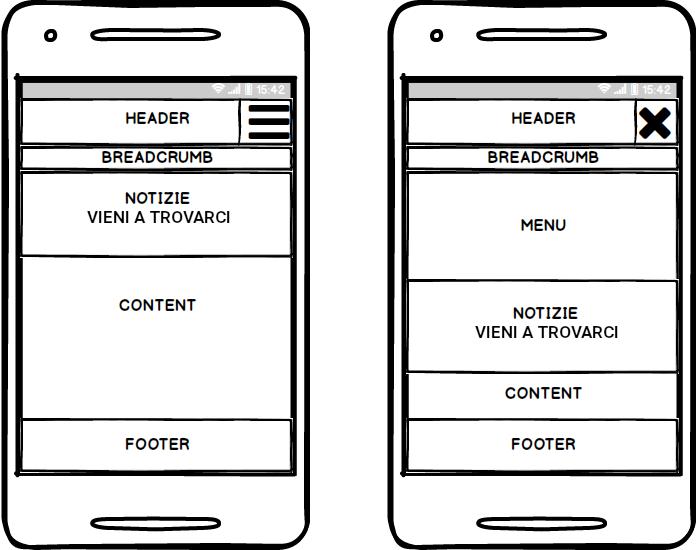
\includegraphics[width=0.7\linewidth]{sezioni/Progettazione/Immagini/mobile_layout.png}
	    \caption{Layout di una pagina in versione mobile: menu chiuso(sinistra) e menu aperto(destra)}
	    \label{Fig:verMobile}
	\end{figure}	  
\end{itemize}
\newpage